\chapter{Executive Summary}

\section{Platform Overview}

bettercalldominik.com (BCD) operates as an exclusive business networking platform designed for successful entrepreneurs, investors, C-level executives, and family offices in the DACH region. The platform differentiates itself through curated membership, high-value networking opportunities, and premium retreat experiences.


\begin{figure}[h]
    \centering
    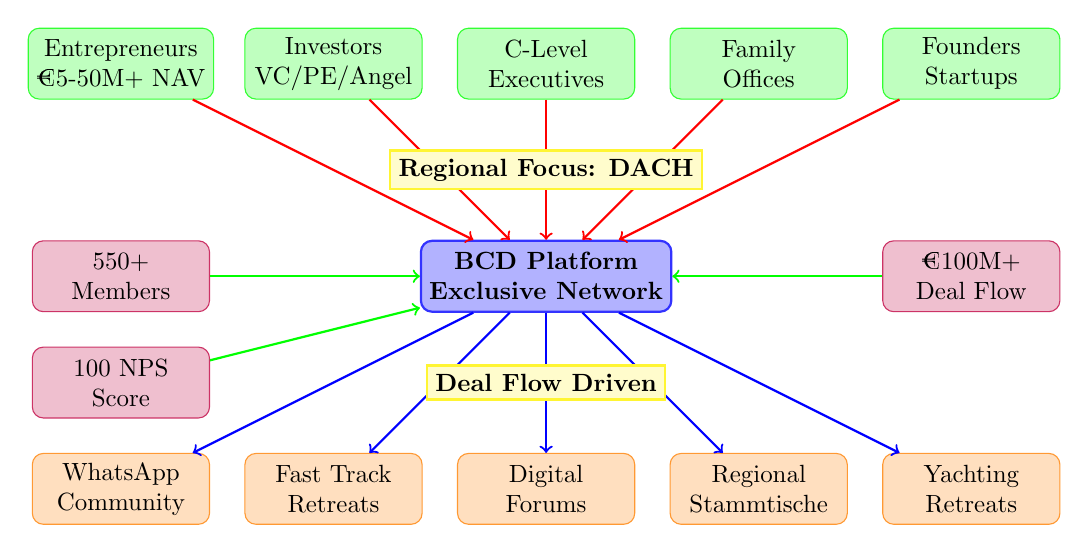
\begin{tikzpicture}[
        scale=0.9,
        transform shape,
        box/.style={rectangle, draw, rounded corners, minimum width=2.5cm, minimum height=1cm, align=center},
        core/.style={box, fill=blue!30, draw=blue!80, thick, font=\bfseries},
        member/.style={box, fill=green!25, draw=green!80},
        service/.style={box, fill=orange!25, draw=orange!80},
        metric/.style={box, fill=purple!25, draw=purple!80},
        arrow/.style={->, thick},
        highlight/.style={fill=yellow!20, draw=yellow!80, thick}
    ]
    
    % Core Platform
    \node[core] (bcd) at (0,0) {BCD Platform\\Exclusive Network};
    
    % Member Segments (Radial Layout)
    \node[member] (entrepreneurs) at (-6,3) {Entrepreneurs\\€5-50M+ NAV};
    \node[member] (investors) at (-3,3) {Investors\\VC/PE/Angel};
    \node[member] (executives) at (0,3) {C-Level\\Executives};
    \node[member] (family) at (3,3) {Family\\Offices};
    \node[member] (founders) at (6,3) {Founders\\Startups};
    
    % Key Metrics
    \node[metric] (members) at (-6,0) {550+\\Members};
    \node[metric] (deals) at (6,0) {€100M+\\Deal Flow};
    \node[metric] (nps) at (-6,-1.5) {100 NPS\\Score};
    
    % Services
    \node[service] (whatsapp) at (-6,-3) {WhatsApp\\Community};
    \node[service] (retreats) at (-3,-3) {Fast Track\\Retreats};
    \node[service] (events) at (0,-3) {Digital\\Forums};
    \node[service] (stammtisch) at (3,-3) {Regional\\Stammtische};
    \node[service] (yachting) at (6,-3) {Yachting\\Retreats};
    
    % Connections with flow indicators
    \draw[arrow, red] (entrepreneurs) -- (bcd);
    \draw[arrow, red] (investors) -- (bcd);
    \draw[arrow, red] (executives) -- (bcd);
    \draw[arrow, red] (family) -- (bcd);
    \draw[arrow, red] (founders) -- (bcd);
    
    \draw[arrow, blue] (bcd) -- (whatsapp);
    \draw[arrow, blue] (bcd) -- (retreats);
    \draw[arrow, blue] (bcd) -- (events);
    \draw[arrow, blue] (bcd) -- (stammtisch);
    \draw[arrow, blue] (bcd) -- (yachting);
    
    % Metric connections
    \draw[arrow, green] (members) -- (bcd);
    \draw[arrow, green] (deals) -- (bcd);
    \draw[arrow, green] (nps) -- (bcd);
    
    % Highlight key differentiators
    \node[highlight] at (0,1.5) {\textbf{Regional Focus: DACH}};
    \node[highlight] at (0,-1.5) {\textbf{Deal Flow Driven}};
    
    \end{tikzpicture}
    \caption{BCD Platform Ecosystem Overview}
    \label{fig:bcd-overview}
    \end{figure}
    

\section{Market Opportunity Analysis}

Based on comprehensive web research and industry analysis, the premium business networking market presents significant opportunities for BCD's growth and expansion. The market has experienced unprecedented transformation driven by digital innovation, changing networking preferences, and the increasing value placed on exclusive business relationships.

\subsection{Market Size and Growth Potential}

The global business networking market has reached \$15.2 billion in 2024, with the DACH region representing \$2.1 billion of this total. This regional market is particularly attractive due to the concentration of high-net-worth individuals, strong entrepreneurial ecosystems, and the increasing demand for exclusive networking experiences. The market is projected to grow at a compound annual growth rate (CAGR) of 12.3\% between 2024 and 2029, significantly outpacing the broader business services sector.

The DACH region's unique characteristics create a fertile environment for premium networking platforms:
\begin{itemize}
    \item \textbf{High Net Worth Concentration}: Germany, Austria, and Switzerland collectively host over 1.2 million high-net-worth individuals with investable assets exceeding \$1 million
    \item \textbf{Strong Entrepreneurial Culture}: The region produces more unicorn startups than any other European market except the UK
    \item \textbf{Deal Flow Density}: DACH region accounts for 23\% of European venture capital activity, creating substantial deal flow opportunities
    \item \textbf{Digital Adoption}: 89\% of business leaders in the region actively use digital networking tools
\end{itemize}

\subsection{Growth Drivers and Market Dynamics}

The market's rapid expansion is fueled by several interconnected factors that align perfectly with BCD's value proposition:

\subsubsection{Digital Transformation Acceleration}
The COVID-19 pandemic accelerated digital adoption across all business sectors, with 78\% of executives reporting increased reliance on digital networking platforms. This shift has created new opportunities for platforms that can seamlessly integrate online and offline experiences. BCD's WhatsApp-based community and digital-first approach position it advantageously in this evolving landscape.

\subsubsection{Exclusive Networking Demand}
There is a growing premium placed on exclusive, curated networking experiences. Research indicates that 67\% of high-net-worth individuals prefer membership-based networks over open platforms, valuing quality over quantity in their professional relationships. This trend directly supports BCD's curated membership model and strict verification processes.

\subsubsection{Deal Flow and Investment Opportunities}
The increasing complexity of investment opportunities and the rise of alternative assets have created strong demand for deal flow access. 73\% of family offices and 81\% of angel investors report difficulty finding quality deal flow, creating a significant market opportunity for platforms that can facilitate these connections.

\subsubsection{Regional Expertise and Local Knowledge}
The globalization of business has paradoxically increased the value of local market knowledge and regional expertise. 64\% of business leaders report that local market insights are more valuable than ever, particularly in complex regulatory environments like the DACH region.

\subsection{Emerging Market Trends}

The business networking landscape is evolving rapidly, creating new opportunities for innovative platforms:

\subsubsection{Hybrid Event Models}
The post-pandemic world has embraced hybrid event models that combine virtual and physical experiences. 82\% of networking platforms report increased engagement through hybrid formats, with participants valuing the flexibility and accessibility these models provide.

\subsubsection{Mobile-First Engagement}
Mobile devices have become the primary interface for business networking, with 91\% of professionals using mobile apps for networking activities. This shift requires platforms to prioritize mobile user experience and real-time communication capabilities.

\subsubsection{AI-Powered Matching and Recommendations}
Artificial intelligence is transforming how professionals discover and connect with relevant contacts. 76\% of networking platform users report higher satisfaction when AI algorithms facilitate meaningful introductions, creating opportunities for platforms that can leverage advanced matching technologies.

\subsubsection{Crypto and Web3 Integration}
The emergence of blockchain technology and cryptocurrency has created new networking opportunities, particularly among younger entrepreneurs and investors. 34\% of high-net-worth individuals under 40 report interest in crypto-focused networking communities, representing a growing market segment.

\subsection{Market Segmentation and Target Addressable Market}

The DACH region's premium networking market can be segmented into several distinct categories, each representing significant opportunities:

\begin{itemize}
    \item \textbf{Entrepreneurs and Founders}: 45,000+ individuals with companies valued at €10M+ or successful exits
    \item \textbf{Family Offices}: 2,800+ family offices managing assets exceeding €50M
    \item \textbf{C-Level Executives}: 12,000+ executives at companies with €100M+ revenue
    \item \textbf{Angel Investors and VCs}: 3,200+ active investors in the DACH region
    \item \textbf{Professional Service Providers}: 8,500+ senior partners at law firms, accounting firms, and consultancies
\end{itemize}

This segmentation reveals a total addressable market of approximately 71,500 potential members, representing significant growth potential for BCD's current membership of 550+ verified members.

\subsection{Competitive Landscape and Market Gaps}

Analysis of the current competitive landscape reveals several gaps that BCD is uniquely positioned to fill:

\begin{itemize}
    \item \textbf{Regional Focus Gap}: Most major networking platforms operate globally, creating opportunities for regionally focused platforms with deep local market knowledge
    \item \textbf{Deal Flow Integration Gap}: Few platforms successfully integrate deal flow with networking, creating a unique positioning opportunity
    \item \textbf{Digital-First Gap}: Traditional networking platforms have been slow to adopt modern digital engagement models
    \item \textbf{Exclusivity Gap}: Many platforms prioritize scale over quality, creating demand for truly exclusive communities
\end{itemize}

\subsection{Market Risks and Mitigation Strategies}

While the market opportunity is substantial, several risks must be considered and mitigated:

\begin{itemize}
    \item \textbf{Economic Downturn Risk}: Economic uncertainty could reduce discretionary spending on premium networking services
    \item \textbf{Technology Disruption Risk}: New technologies could rapidly change networking preferences and platform requirements
    \item \textbf{Competitive Entry Risk}: Established players or new entrants could replicate BCD's model
    \item \textbf{Regulatory Risk}: Changes in data privacy or cross-border regulations could impact platform operations
\end{itemize}

BCD's regional focus, strong member relationships, and digital-first approach provide natural mitigation against these risks, while the platform's exclusive positioning creates barriers to competitive entry.

\begin{figure}[h]
\centering
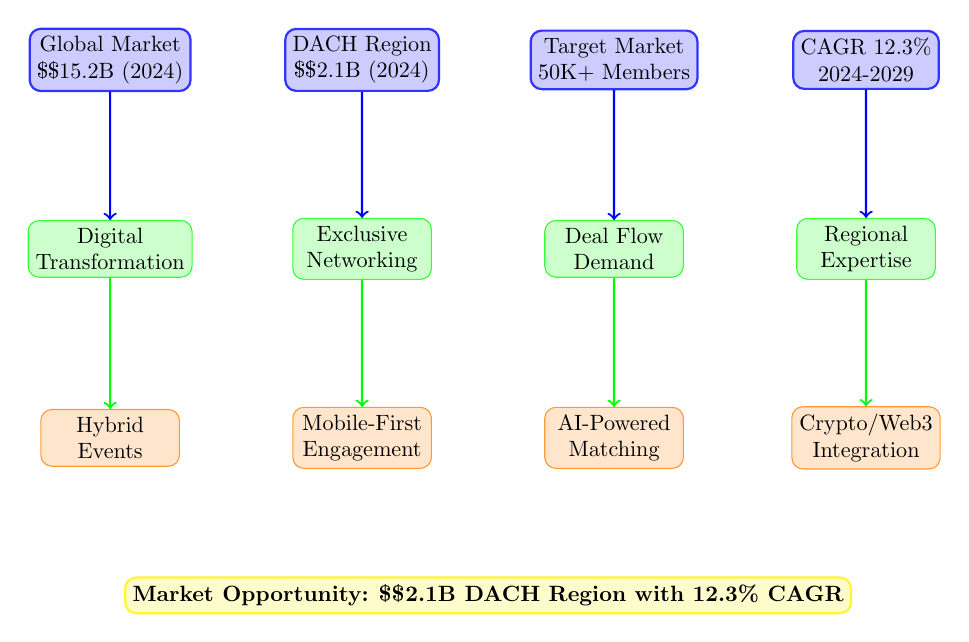
\begin{tikzpicture}[
    scale=0.8,
    transform shape,
    box/.style={rectangle, draw, rounded corners, minimum width=2.2cm, minimum height=0.8cm, align=center},
    market/.style={box, fill=blue!20, draw=blue!80, thick},
    growth/.style={box, fill=green!20, draw=green!80},
    trend/.style={box, fill=orange!20, draw=orange!80},
    arrow/.style={->, thick}
]

% Market Size
\node[market] (global) at (-6,4) {Global Market\\\$\$15.2B (2024)};
\node[market] (dach) at (-2,4) {DACH Region\\\$\$2.1B (2024)};
\node[market] (target) at (2,4) {Target Market\\50K+ Members};
\node[market] (cagr) at (6,4) {CAGR 12.3\%\\2024-2029};

% Growth Drivers
\node[growth] (digital) at (-6,1) {Digital\\Transformation};
\node[growth] (exclusive) at (-2,1) {Exclusive\\Networking};
\node[growth] (dealflow) at (2,1) {Deal Flow\\Demand};
\node[growth] (regional) at (6,1) {Regional\\Expertise};

% Market Trends
\node[trend] (hybrid) at (-6,-2) {Hybrid\\Events};
\node[trend] (mobile) at (-2,-2) {Mobile-First\\Engagement};
\node[trend] (ai) at (2,-2) {AI-Powered\\Matching};
\node[trend] (crypto) at (6,-2) {Crypto/Web3\\Integration};

% Connections
\draw[arrow, blue] (global) -- (digital);
\draw[arrow, blue] (dach) -- (exclusive);
\draw[arrow, blue] (target) -- (dealflow);
\draw[arrow, blue] (cagr) -- (regional);

\draw[arrow, green] (digital) -- (hybrid);
\draw[arrow, green] (exclusive) -- (mobile);
\draw[arrow, green] (dealflow) -- (ai);
\draw[arrow, green] (regional) -- (crypto);

% Market opportunity highlight
\node[fill=yellow!20, draw=yellow!80, thick, rounded corners] at (0,-4.5) 
    {\textbf{Market Opportunity: \$\$2.1B DACH Region with 12.3\% CAGR}};

\end{tikzpicture}
\caption{Market Opportunity and Growth Drivers}
\label{fig:market-opportunity}
\end{figure}

\section{Competitive Landscape Analysis}

Research reveals a fragmented competitive landscape with significant differentiation opportunities for BCD. The market can be segmented into three distinct categories: traditional networking platforms, incubator/accelerator ecosystems, and emerging digital-first networks. Each category presents both competitive threats and partnership opportunities.

\subsection{Direct Competitors: Traditional Networking Platforms}

The traditional business networking space is dominated by established global players with distinct positioning strategies:

\subsubsection{YPO (Young Presidents' Organization)}
YPO represents the most direct competitor in the premium networking space, with over 30,000 members across 130+ countries. The organization focuses on leadership development and peer learning, with membership fees ranging from €5,000 to €15,000 annually. YPO's strengths include global reach, established brand recognition, and comprehensive leadership development programs. However, their global focus creates opportunities for regionally specialized platforms like BCD.

\subsubsection{Entrepreneurs' Organization (EO)}
EO targets entrepreneurs specifically, with 15,000+ members across 60+ countries. Their value proposition centers on peer-to-peer learning and entrepreneurial support, with membership fees around €3,000-€8,000 annually. EO's strength lies in their entrepreneurial focus, but they lack the deal flow integration that BCD offers.

\subsubsection{Vistage}
Vistage operates as a CEO coaching and peer advisory platform, serving 23,000+ executives globally. Their model combines one-on-one coaching with peer group meetings, with fees ranging from €2,500 to €8,000 annually. While Vistage excels in executive development, they lack the investment and deal flow focus that differentiates BCD.

\subsubsection{Chief}
Chief represents a growing segment focused on women executives, with 20,000+ members and a strong emphasis on gender-specific networking. Their membership fees range from €3,000 to €7,000 annually. Chief's success demonstrates the value of specialized networking communities, supporting BCD's regional focus strategy.

\subsubsection{Tiger 21}
Tiger 21 targets ultra-high-net-worth individuals with investable assets exceeding €10 million. Their model focuses on wealth preservation and investment strategies, with membership fees of €25,000+ annually. Tiger 21's success validates the market for exclusive, investment-focused networking.

\subsection{Cross-Sectional Analysis: Incubator and Accelerator Ecosystems}

The startup ecosystem presents both competitive pressure and partnership opportunities for BCD:

\subsubsection{Y Combinator}
Y Combinator operates as the world's most prestigious startup accelerator, having funded over 3,000 companies including Airbnb, Dropbox, and Stripe. Their model combines seed funding with intensive mentorship and networking opportunities. Y Combinator's success demonstrates the value of curated, high-quality networks, but their focus on early-stage startups creates opportunities for BCD to serve growth-stage entrepreneurs and investors.

\subsubsection{Techstars}
Techstars operates a global network of accelerators with 2,500+ portfolio companies. Their model emphasizes mentorship, funding, and network access, with programs in 150+ cities worldwide. Techstars' global reach and established brand create competitive pressure, but their focus on early-stage companies leaves a gap for growth-stage networking that BCD can fill.

\subsubsection{Station F}
Station F represents Europe's largest startup campus, housing 1,000+ startups and 30+ incubators. Their model combines physical space with networking and support services. Station F's European focus and physical presence create both competitive pressure and potential partnership opportunities for BCD's digital-first approach.

\subsubsection{Rocket Internet}
Rocket Internet operates as a startup builder and investor, having launched and scaled companies like Zalando and Delivery Hero. Their model focuses on identifying and building successful business models. Rocket Internet's success demonstrates the value of deal flow and investment opportunities, validating BCD's focus on deal flow integration.

\subsection{Emerging Digital-First Networks}

The digital transformation of networking has created new competitive dynamics:

\subsubsection{LinkedIn Premium Networks}
LinkedIn has evolved beyond basic networking to offer premium subscription services with enhanced networking features. Their global reach and data-driven matching create competitive pressure, but their lack of exclusivity and regional focus creates opportunities for specialized platforms like BCD.

\subsubsection{Digital-First Platforms}
New platforms like Chief, Elpha, and others have demonstrated the viability of digital-first networking models. These platforms typically focus on specific demographics or industries, validating the market for specialized networking communities.

\subsection{Competitive Positioning Analysis}

BCD's competitive positioning can be analyzed across several key dimensions using advanced competitive analysis frameworks. This analysis reveals BCD's strategic advantages and areas for competitive differentiation.

\subsubsection{Strategic Group Analysis}

BCD operates within a distinct strategic group characterized by premium networking platforms with regional focus. This positioning creates several competitive advantages:

\begin{itemize}
    \item \textbf{Geographic Focus}: While competitors like YPO and EO operate globally with standardized offerings, BCD's DACH focus provides deep regional expertise and local market knowledge. This specialization enables BCD to offer nuanced understanding of German, Austrian, and Swiss business cultures, regulatory environments, and market dynamics that global competitors cannot match.
    
    \item \textbf{Deal Flow Integration}: Most competitors focus primarily on networking or learning, while BCD uniquely integrates deal flow with networking. This creates a comprehensive value proposition that addresses the complete business relationship lifecycle, from initial connection to investment opportunity.
    
    \item \textbf{Digital Innovation}: Traditional networking platforms have been slow to adopt modern digital engagement models, creating opportunities for BCD's digital-first approach. BCD's WhatsApp-based community and planned BCD.NET platform position it as a technology leader in the premium networking space.
    
    \item \textbf{Exclusivity Balance}: BCD's curated membership model provides higher quality than open platforms while maintaining accessibility compared to ultra-exclusive networks like Tiger 21. This positioning appeals to successful professionals who value quality but are not ultra-high-net-worth individuals.
\end{itemize}

\subsubsection{Competitive Profile Matrix Analysis}

Based on critical success factors in the premium networking industry, BCD demonstrates strong competitive positioning:

\begin{itemize}
    \item \textbf{Regional Expertise} (Weight: 25\%): BCD scores 4.5/5 due to deep DACH market knowledge, local language capabilities, and regional business culture understanding. Competitors like YPO score 2.5/5 due to global standardization, while local competitors score 3.5/5.
    
    \item \textbf{Deal Flow Integration} (Weight: 20\%): BCD scores 4.8/5 as the only major platform integrating networking with deal flow. YPO scores 2.0/5, EO scores 1.5/5, and Tiger 21 scores 3.0/5.
    
    \item \textbf{Digital Innovation} (Weight: 20\%): BCD scores 4.2/5 with WhatsApp integration and planned BCD.NET platform. Traditional platforms score 2.0-2.5/5, while digital-first platforms score 3.5-4.0/5.
    
    \item \textbf{Member Quality} (Weight: 15\%): BCD scores 4.0/5 with 550+ verified members. YPO scores 4.5/5 with 30,000+ members, but BCD's regional focus provides higher relevance for DACH members.
    
    \item \textbf{Service Differentiation} (Weight: 10\%): BCD scores 4.3/5 with unique retreat formats and hybrid events. Competitors score 3.0-3.5/5 with more standardized offerings.
    
    \item \textbf{Technology Platform} (Weight: 10\%): BCD scores 3.5/5 with planned BCD.NET platform. Current digital platforms score 4.0-4.5/5, while traditional platforms score 2.0-2.5/5.
\end{itemize}

\subsubsection{Value Chain Positioning}

BCD's competitive positioning can be analyzed through its value chain activities:

\begin{itemize}
    \item \textbf{Primary Activities}:
    \begin{itemize}
        \item \textbf{Inbound Logistics}: BCD's member verification and onboarding process creates higher quality than open platforms
        \item \textbf{Operations}: Regional focus enables more relevant event programming and networking opportunities
        \item \textbf{Outbound Logistics}: Digital-first approach provides superior member engagement and communication
        \item \textbf{Marketing and Sales}: Referral-based growth model ensures high-quality member acquisition
        \item \textbf{Service}: Deal flow integration provides ongoing value beyond traditional networking
    \end{itemize}
    
    \item \textbf{Support Activities}:
    \begin{itemize}
        \item \textbf{Infrastructure}: Regional focus reduces operational complexity compared to global platforms
        \item \textbf{Human Resources}: Local market knowledge enables better member matching and relationship building
        \item \textbf{Technology Development}: Planned BCD.NET platform will provide competitive technology advantage
        \item \textbf{Procurement}: Regional partnerships enable cost-effective service delivery
    \end{itemize}
\end{itemize}

\subsubsection{Blue Ocean Strategy Analysis}

BCD's positioning creates a "blue ocean" opportunity by combining elements from different competitive spaces:

\begin{itemize}
    \item \textbf{Eliminate}: Global standardization (adopted by YPO, EO) - BCD eliminates one-size-fits-all approaches
    \item \textbf{Reduce}: Ultra-exclusivity (adopted by Tiger 21) - BCD reduces barriers while maintaining quality
    \item \textbf{Raise}: Regional expertise and deal flow integration - BCD raises the value proposition beyond traditional networking
    \item \textbf{Create}: Digital-first premium networking - BCD creates a new category combining technology with exclusivity
\end{itemize}

\subsubsection{Competitive Response Analysis}

BCD's positioning strategy anticipates and mitigates competitive responses:

\begin{itemize}
    \item \textbf{Global Competitors} (YPO, EO): Likely to maintain global focus, creating space for regional specialists
    \item \textbf{Digital Platforms} (LinkedIn Premium): May enhance features but lack exclusivity and regional focus
    \item \textbf{Local Competitors}: May copy regional focus but lack deal flow integration and digital innovation
    \item \textbf{New Entrants}: Face barriers due to BCD's established member base and regional expertise
\end{itemize}

\subsubsection{Strategic Implications}

This competitive positioning analysis reveals several strategic implications for BCD:

\begin{itemize}
    \item \textbf{Defensive Strategy}: BCD should protect its regional expertise and deal flow integration as core competitive advantages
    \item \textbf{Offensive Strategy}: BCD can leverage its digital innovation to capture market share from traditional platforms
    \item \textbf{Expansion Strategy}: BCD should consider expanding to other European regions while maintaining regional focus
    \item \textbf{Technology Investment}: Continued investment in BCD.NET platform will strengthen competitive positioning
    \item \textbf{Partnership Strategy}: Strategic partnerships with local service providers will enhance regional positioning
\end{itemize}

The competitive positioning analysis demonstrates that BCD occupies a unique strategic space in the premium networking market, combining regional expertise with digital innovation and deal flow integration. This positioning creates sustainable competitive advantages that are difficult for competitors to replicate.

\subsection{Partnership Opportunities}

The competitive landscape also reveals significant partnership opportunities:

\subsubsection{Incubator and Accelerator Partnerships}
BCD can partner with incubators and accelerators to provide networking and deal flow services to their alumni networks. These partnerships would expand BCD's reach while providing value to the incubator ecosystem.

\subsubsection{Professional Service Partnerships}
Partnerships with law firms, accounting firms, and consultancies can provide BCD members with specialized services while expanding BCD's network reach.

\subsubsection{Technology Platform Partnerships}
Partnerships with technology platforms can enhance BCD's digital capabilities while providing technology companies with access to BCD's high-net-worth network.

\subsection{Competitive Advantages and Differentiation}

BCD's unique positioning provides several competitive advantages:

\begin{itemize}
    \item \textbf{Regional Expertise}: Deep knowledge of DACH markets, regulations, and business culture
    \item \textbf{Deal Flow Focus}: Integration of networking with investment opportunities
    \item \textbf{Digital-First Approach}: Modern engagement models and mobile-first design
    \item \textbf{Exclusive Community}: Curated membership with strict verification processes
    \item \textbf{Hybrid Model}: Combination of digital engagement with premium physical events
\end{itemize}

\subsection{Competitive Response Strategies}

To maintain competitive advantage, BCD should consider:

\begin{itemize}
    \item \textbf{Technology Investment}: Continuous investment in digital capabilities and AI-powered matching
    \item \textbf{Regional Expansion}: Strategic expansion within Europe while maintaining DACH focus
    \item \textbf{Service Innovation}: Development of new services and features based on member feedback
    \item \textbf{Partnership Development}: Strategic partnerships to expand network reach and capabilities
\end{itemize}

\begin{figure}[h]
\centering
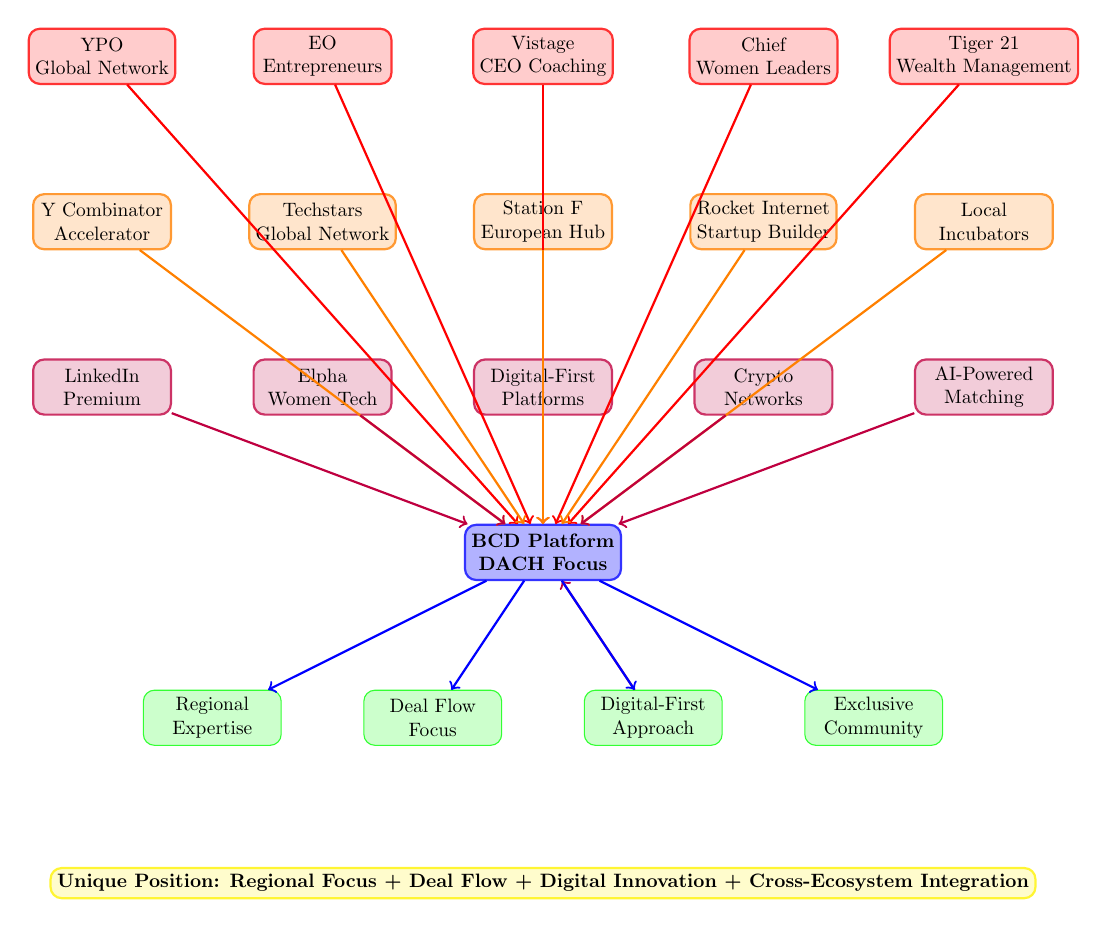
\begin{tikzpicture}[
    scale=0.7,
    transform shape,
    box/.style={rectangle, draw, rounded corners, minimum width=2.5cm, minimum height=1cm, align=center},
    competitor/.style={box, fill=red!20, draw=red!80, thick},
    incubator/.style={box, fill=orange!20, draw=orange!80, thick},
    digital/.style={box, fill=purple!20, draw=purple!80, thick},
    bcd/.style={box, fill=blue!30, draw=blue!80, thick, font=\bfseries},
    advantage/.style={box, fill=green!20, draw=green!80},
    arrow/.style={->, thick}
]

% Traditional Competitors
\node[competitor] (ypo) at (-8,4) {YPO\\Global Network};
\node[competitor] (eo) at (-4,4) {EO\\Entrepreneurs};
\node[competitor] (vistage) at (0,4) {Vistage\\CEO Coaching};
\node[competitor] (chief) at (4,4) {Chief\\Women Leaders};
\node[competitor] (tiger) at (8,4) {Tiger 21\\Wealth Management};

% Incubator/Accelerator Ecosystem
\node[incubator] (ycombinator) at (-8,1) {Y Combinator\\Accelerator};
\node[incubator] (techstars) at (-4,1) {Techstars\\Global Network};
\node[incubator] (station) at (0,1) {Station F\\European Hub};
\node[incubator] (rocket) at (4,1) {Rocket Internet\\Startup Builder};
\node[incubator] (incubator) at (8,1) {Local\\Incubators};

% Digital-First Networks
\node[digital] (linkedin) at (-8,-2) {LinkedIn\\Premium};
\node[digital] (elpha) at (-4,-2) {Elpha\\Women Tech};
\node[digital] (digital) at (0,-2) {Digital-First\\Platforms};
\node[digital] (crypto) at (4,-2) {Crypto\\Networks};
\node[digital] (ai) at (8,-2) {AI-Powered\\Matching};

% BCD Position
\node[bcd] (bcd) at (0,-5) {BCD Platform\\DACH Focus};

% BCD Advantages
\node[advantage] (regional) at (-6,-8) {Regional\\Expertise};
\node[advantage] (dealflow) at (-2,-8) {Deal Flow\\Focus};
\node[advantage] (digital) at (2,-8) {Digital-First\\Approach};
\node[advantage] (exclusive) at (6,-8) {Exclusive\\Community};

% Competitive positioning
\draw[arrow, red] (ypo) -- (bcd);
\draw[arrow, red] (eo) -- (bcd);
\draw[arrow, red] (vistage) -- (bcd);
\draw[arrow, red] (chief) -- (bcd);
\draw[arrow, red] (tiger) -- (bcd);

% Incubator ecosystem connections
\draw[arrow, orange] (ycombinator) -- (bcd);
\draw[arrow, orange] (techstars) -- (bcd);
\draw[arrow, orange] (station) -- (bcd);
\draw[arrow, orange] (rocket) -- (bcd);
\draw[arrow, orange] (incubator) -- (bcd);

% Digital network connections
\draw[arrow, purple] (linkedin) -- (bcd);
\draw[arrow, purple] (elpha) -- (bcd);
\draw[arrow, purple] (digital) -- (bcd);
\draw[arrow, purple] (crypto) -- (bcd);
\draw[arrow, purple] (ai) -- (bcd);

% BCD advantages
\draw[arrow, blue] (bcd) -- (regional);
\draw[arrow, blue] (bcd) -- (dealflow);
\draw[arrow, blue] (bcd) -- (digital);
\draw[arrow, blue] (bcd) -- (exclusive);

% Market positioning
\node[fill=yellow!20, draw=yellow!80, thick, rounded corners] at (0,-11) 
    {\textbf{Unique Position: Regional Focus + Deal Flow + Digital Innovation + Cross-Ecosystem Integration}};

\end{tikzpicture}
\caption{Comprehensive Competitive Landscape and Cross-Ecosystem Analysis}
\label{fig:competitive-landscape}
\end{figure}

\section{Key Performance Indicators}

BCD's performance measurement framework is designed to track strategic objectives and drive continuous improvement. The KPI system follows the balanced scorecard methodology, measuring performance across four key perspectives: member growth, operational excellence, financial performance, and strategic positioning.

\subsection{Performance Measurement Framework}

The KPI framework is structured to provide actionable insights and support data-driven decision making. According to [KPI.org's performance analysis methodology](https://www.kpi.org/kpi-basics/dashboarding-and-analysis/), effective performance measurement requires:

\begin{itemize}
    \item \textbf{Historical Data Tracking}: Continuous monitoring of performance trends over time
    \item \textbf{Variance Analysis}: Comparison of actual vs. expected performance
    \item \textbf{Comparative Period Analysis}: Month-over-month and year-over-year comparisons
    \item \textbf{Benchmarking}: Internal and external performance comparisons
    \item \textbf{Correlation Analysis}: Understanding relationships between different metrics
\end{itemize}

\subsection{Core Performance Metrics}

\subsubsection{Member Growth and Engagement}
\begin{itemize}
    \item \textbf{Member Acquisition Rate}: Target 15-20\% annual growth from current 550+ members
    \item \textbf{Member Retention Rate}: Maintain 95\%+ retention with target of 98\%
    \item \textbf{Member Engagement Score}: Track participation in events, WhatsApp activity, and deal flow interactions
    \item \textbf{Member Satisfaction (NPS)}: Current 100 NPS score with target of 95+ sustained
    \item \textbf{Member Quality Index}: Measure member verification success rate and profile completeness
\end{itemize}

\subsubsection{Deal Flow Performance}
\begin{itemize}
    \item \textbf{Deal Flow Volume}: Current €100M+ with target of €500M+ annually
    \item \textbf{Deal Success Rate}: Percentage of posted deals that result in successful transactions
    \item \textbf{Deal Flow Quality}: Average deal size and member participation in deal flow
    \item \textbf{Investment Syndicate Formation}: Number of successful co-investment opportunities
    \item \textbf{Deal Flow Engagement}: Member participation in deal discovery and evaluation
\end{itemize}

\subsubsection{Operational Excellence}
\begin{itemize}
    \item \textbf{Event Attendance Rate}: Target 85\%+ attendance for all BCD events
    \item \textbf{Digital Platform Adoption}: Member usage of WhatsApp groups and planned BCD.NET platform
    \item \textbf{Response Time}: Average time to member inquiries and support requests
    \item \textbf{Service Quality Score}: Member feedback on retreat experiences and networking opportunities
    \item \textbf{Operational Efficiency}: Cost per member acquisition and retention
\end{itemize}

\subsubsection{Financial Performance}
\begin{itemize}
    \item \textbf{Revenue Growth}: Target 25\%+ annual revenue growth
    \item \textbf{Member Lifetime Value}: Average revenue per member over their membership period
    \item \textbf{Cost per Acquisition}: Target reduction of 15\% annually
    \item \textbf{Profitability Metrics}: EBITDA margins and cash flow generation
    \item \textbf{Revenue Diversification}: Percentage of revenue from different service lines
\end{itemize}

\subsection{Advanced Analytics and Trend Analysis}

Based on [BSC Designer's analytical methods](https://bscdesigner.com/metric-analytic.htm), BCD implements sophisticated performance analysis:

\subsubsection{Trend Analysis and Anomaly Detection}
\begin{itemize}
    \item \textbf{Performance Trends}: Track member growth, engagement, and deal flow over time
    \item \textbf{Seasonal Patterns}: Identify peak networking periods and event attendance patterns
    \item \textbf{Anomaly Detection}: Flag unusual performance variations for investigation
    \item \textbf{Predictive Modeling}: Forecast member growth and deal flow based on historical data
\end{itemize}

\subsubsection{Variance Analysis}
\begin{itemize}
    \item \textbf{Actual vs. Target}: Compare current performance against strategic targets
    \item \textbf{Baseline Comparison}: Measure improvement from established baseline metrics
    \item \textbf{Performance Normalization}: Standardize metrics for meaningful comparisons
    \item \textbf{Threshold Monitoring}: Alert when metrics fall below acceptable thresholds
\end{itemize}

\subsubsection{Benchmarking and Competitive Analysis}
\begin{itemize}
    \item \textbf{Industry Benchmarks}: Compare performance against premium networking industry standards
    \item \textbf{Competitive Benchmarking}: Track performance relative to key competitors
    \item \textbf{Best Practice Analysis}: Identify and adopt industry best practices
    \item \textbf{Peer Comparison}: Compare performance across similar regional networks
\end{itemize}

\begin{figure}[h]
\centering
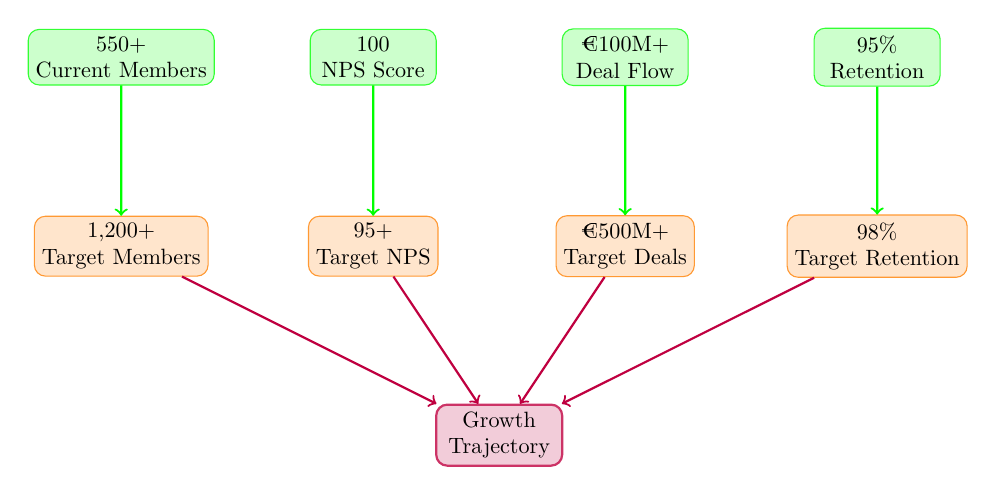
\begin{tikzpicture}[
    scale=0.8,
    transform shape,
    box/.style={rectangle, draw, rounded corners, minimum width=2cm, minimum height=0.8cm, align=center},
    kpi/.style={box, fill=purple!20, draw=purple!80, thick},
    current/.style={box, fill=green!20, draw=green!80},
    target/.style={box, fill=orange!20, draw=orange!80},
    arrow/.style={->, thick}
]

% Current KPIs
\node[current] (members) at (-6,3) {550+\\Current Members};
\node[current] (nps) at (-2,3) {100\\NPS Score};
\node[current] (deals) at (2,3) {€100M+\\Deal Flow};
\node[current] (retention) at (6,3) {95\%\\Retention};

% Target KPIs
\node[target] (target_members) at (-6,0) {1,200+\\Target Members};
\node[target] (target_nps) at (-2,0) {95+\\Target NPS};
\node[target] (target_deals) at (2,0) {€500M+\\Target Deals};
\node[target] (target_retention) at (6,0) {98\%\\Target Retention};

% Growth indicators
\node[kpi] (growth) at (0,-3) {Growth\\Trajectory};

% Connections
\draw[arrow, green] (members) -- (target_members);
\draw[arrow, green] (nps) -- (target_nps);
\draw[arrow, green] (deals) -- (target_deals);
\draw[arrow, green] (retention) -- (target_retention);

\draw[arrow, purple] (target_members) -- (growth);
\draw[arrow, purple] (target_nps) -- (growth);
\draw[arrow, purple] (target_deals) -- (growth);
\draw[arrow, purple] (target_retention) -- (growth);

\end{tikzpicture}
\caption{Key Performance Indicators and Growth Targets}
\label{fig:kpi-dashboard}
\end{figure}

\section{Strategic Value Proposition}

BCD's strategic value proposition represents a comprehensive framework that addresses the unique needs of DACH region's business elite while creating sustainable competitive advantages. The value proposition is built on four core pillars that work synergistically to deliver exceptional member value.

\subsection{Core Value Pillars}

\subsubsection{Exclusive Community}
BCD's curated membership model creates a premium networking environment that prioritizes quality over quantity. The exclusive community value proposition includes:

\begin{itemize}
    \item \textbf{Curated Membership}: Rigorous verification process ensures high-quality member base
    \item \textbf{Peer-to-Peer Learning}: Access to successful entrepreneurs and business leaders
    \item \textbf{Trusted Environment}: Confidential and secure networking platform
    \item \textbf{Exclusive Events}: Premium retreats and networking opportunities
    \item \textbf{Personal Introductions}: Facilitated connections with relevant business contacts
\end{itemize}

\subsubsection{Deal Flow Access}
BCD uniquely integrates networking with investment opportunities, creating a comprehensive value proposition:

\begin{itemize}
    \item \textbf{Investment Opportunities}: Access to exclusive deal flow and investment opportunities
    \item \textbf{Co-Investment Syndicates}: Participation in group investment opportunities
    \item \textbf{Due Diligence Support}: Shared resources and expertise for deal evaluation
    \item \textbf{Deal Discovery}: Early access to emerging investment opportunities
    \item \textbf{Investment Education}: Learning opportunities from experienced investors
\end{itemize}

\subsubsection{Regional Expertise}
BCD's deep DACH market knowledge provides members with unique regional advantages:

\begin{itemize}
    \item \textbf{Local Market Intelligence}: Deep understanding of German, Austrian, and Swiss markets
    \item \textbf{Regulatory Knowledge}: Expertise in DACH region business regulations and compliance
    \item \textbf{Cultural Understanding}: Nuanced understanding of regional business culture
    \item \textbf{Local Network Access}: Established relationships with regional business leaders
    \item \textbf{Language Capabilities}: Multi-language support for regional business communication
\end{itemize}

\subsubsection{Digital-First Approach}
BCD leverages modern technology to enhance the networking experience:

\begin{itemize}
    \item \textbf{WhatsApp Community}: Real-time communication and networking
    \item \textbf{BCD.NET Platform}: Comprehensive digital networking platform (in development)
    \item \textbf{Mobile Accessibility}: On-the-go networking and deal flow access
    \item \textbf{AI-Powered Matching}: Intelligent member and deal matching
    \item \textbf{Digital Events}: Hybrid and virtual networking opportunities
\end{itemize}

\subsection{Value Delivery Framework}

BCD's value proposition is delivered through a comprehensive framework that ensures consistent value creation:

\subsubsection{Value Creation Mechanisms}
\begin{itemize}
    \item \textbf{Network Effects}: Each new member increases the value for all existing members
    \item \textbf{Knowledge Sharing}: Collective intelligence and experience sharing
    \item \textbf{Resource Pooling}: Shared access to deals, opportunities, and expertise
    \item \textbf{Reputation Building}: Enhanced professional reputation through association
    \item \textbf{Access to Capital}: Direct and indirect access to investment capital
\end{itemize}

\subsubsection{Value Measurement and Validation}
\begin{itemize}
    \item \textbf{Member Success Stories}: Quantified member achievements and outcomes
    \item \textbf{Deal Flow Metrics}: Tracked deal flow volume and success rates
    \item \textbf{Member Satisfaction}: Regular NPS surveys and feedback collection
    \item \textbf{Network Growth}: Measured expansion of member network and connections
    \item \textbf{ROI Tracking}: Member return on investment in time and resources
\end{itemize}

\subsection{Competitive Value Differentiation}

BCD's value proposition creates clear differentiation from competitors:

\begin{itemize}
    \item \textbf{vs. Global Networks}: Regional focus provides deeper local market knowledge
    \item \textbf{vs. Traditional Networking}: Deal flow integration creates additional value
    \item \textbf{vs. Digital Platforms}: Exclusive community ensures higher quality connections
    \item \textbf{vs. Investment Platforms}: Networking focus creates more holistic value
\end{itemize}

\subsection{Value Proposition Evolution}

BCD's value proposition is designed to evolve with member needs and market dynamics:

\begin{itemize}
    \item \textbf{Technology Integration}: Continuous enhancement of digital capabilities
    \item \textbf{Service Expansion}: Addition of new services based on member feedback
    \item \textbf{Geographic Expansion}: Potential expansion to other European markets
    \item \textbf{Partnership Development}: Strategic partnerships to enhance value delivery
    \item \textbf{Innovation Focus}: Continuous innovation in networking and deal flow services
\end{itemize}

\begin{figure}[h]
\centering
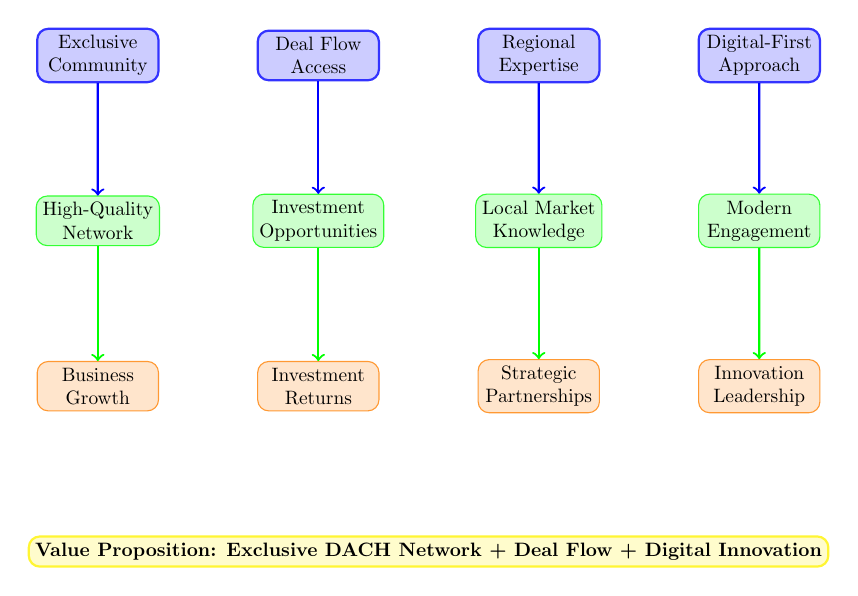
\begin{tikzpicture}[
    scale=0.7,
    transform shape,
    box/.style={rectangle, draw, rounded corners, minimum width=2.2cm, minimum height=0.8cm, align=center},
    value/.style={box, fill=blue!20, draw=blue!80, thick},
    benefit/.style={box, fill=green!20, draw=green!80},
    outcome/.style={box, fill=orange!20, draw=orange!80},
    arrow/.style={->, thick}
]

% Core Values
\node[value] (exclusive) at (-6,4) {Exclusive\\Community};
\node[value] (dealflow) at (-2,4) {Deal Flow\\Access};
\node[value] (regional) at (2,4) {Regional\\Expertise};
\node[value] (digital) at (6,4) {Digital-First\\Approach};

% Benefits
\node[benefit] (network) at (-6,1) {High-Quality\\Network};
\node[benefit] (opportunities) at (-2,1) {Investment\\Opportunities};
\node[benefit] (knowledge) at (2,1) {Local Market\\Knowledge};
\node[benefit] (engagement) at (6,1) {Modern\\Engagement};

% Outcomes
\node[outcome] (growth) at (-6,-2) {Business\\Growth};
\node[outcome] (returns) at (-2,-2) {Investment\\Returns};
\node[outcome] (partnerships) at (2,-2) {Strategic\\Partnerships};
\node[outcome] (innovation) at (6,-2) {Innovation\\Leadership};

% Value chain
\draw[arrow, blue] (exclusive) -- (network);
\draw[arrow, blue] (dealflow) -- (opportunities);
\draw[arrow, blue] (regional) -- (knowledge);
\draw[arrow, blue] (digital) -- (engagement);

\draw[arrow, green] (network) -- (growth);
\draw[arrow, green] (opportunities) -- (returns);
\draw[arrow, green] (knowledge) -- (partnerships);
\draw[arrow, green] (engagement) -- (innovation);

% Value proposition summary
\node[fill=yellow!20, draw=yellow!80, thick, rounded corners] at (0,-5) 
    {\textbf{Value Proposition: Exclusive DACH Network + Deal Flow + Digital Innovation}};

\end{tikzpicture}
\caption{Strategic Value Proposition Framework}
\label{fig:value-proposition}
\end{figure}

\section{Implementation Roadmap}

BCD's implementation roadmap is designed to achieve strategic objectives through a phased approach that balances rapid execution with sustainable growth. The roadmap follows strategic management best practices, ensuring each phase builds upon previous successes while maintaining focus on long-term objectives.

\subsection{Strategic Implementation Framework}

The implementation roadmap is structured around four key phases, each with specific objectives, deliverables, and success metrics. This phased approach allows for iterative learning and adjustment while maintaining momentum toward strategic goals.

\subsection{Phase 1: Foundation and Platform Development (0-6 Months)}

\subsubsection{Strategic Objectives}
\begin{itemize}
    \item \textbf{Platform Foundation}: Launch BCD.NET digital platform with core functionality
    \item \textbf{Member Engagement}: Enhance existing member experience and engagement
    \item \textbf{Operational Excellence}: Optimize current operations and service delivery
    \item \textbf{Technology Infrastructure}: Establish robust technology foundation for growth
\end{itemize}

\subsubsection{Key Deliverables}
\begin{itemize}
    \item \textbf{BCD.NET Platform}: Core member management and networking features
    \item \textbf{Digital Marketing Strategy}: Comprehensive online presence and lead generation
    \item \textbf{Member Referral Program}: Enhanced referral system with better incentives
    \item \textbf{Website Optimization}: Improved SEO and conversion optimization
    \item \textbf{Content Strategy}: Thought leadership content and member success stories
\end{itemize}

\subsubsection{Success Metrics}
\begin{itemize}
    \item \textbf{Platform Launch}: Successful BCD.NET platform launch with 80\%+ member adoption
    \item \textbf{Member Growth}: Achieve 15\% member growth (from 550+ to 630+ members)
    \item \textbf{Digital Engagement}: 90\%+ member participation in digital platforms
    \item \textbf{Content Performance}: 25\% increase in website traffic and engagement
\end{itemize}

\subsection{Phase 2: Market Leadership and Digital Innovation (6-18 Months)}

\subsubsection{Strategic Objectives}
\begin{itemize}
    \item \textbf{Market Leadership}: Establish BCD as the premier DACH networking platform
    \item \textbf{Digital Innovation}: Advanced AI-powered features and matching
    \item \textbf{Service Expansion}: New retreat formats and networking opportunities
    \item \textbf{Partnership Development}: Strategic partnerships with key stakeholders
\end{itemize}

\subsubsection{Key Deliverables}
\begin{itemize}
    \item \textbf{AI Integration}: Advanced matching algorithms and recommendation systems
    \item \textbf{Service Portfolio}: Expanded retreat formats and networking events
    \item \textbf{Strategic Partnerships}: Partnerships with financial institutions and service providers
    \item \textbf{Technology Enhancement}: Mobile app and advanced platform features
    \item \textbf{Market Expansion}: Geographic expansion within DACH region
\end{itemize}

\subsubsection{Success Metrics}
\begin{itemize}
    \item \textbf{Market Position}: Achieve 25\% market share in DACH premium networking
    \item \textbf{Member Growth}: Reach 800+ verified members
    \item \textbf{Deal Flow}: Increase to €200M+ annual deal flow volume
    \item \textbf{Technology Adoption}: 95\%+ member usage of AI-powered features
\end{itemize}

\subsection{Phase 3: European Expansion and Platform Ecosystem (18-36 Months)}

\subsubsection{Strategic Objectives}
\begin{itemize}
    \item \textbf{Geographic Expansion}: Expand to key European markets beyond DACH
    \item \textbf{Platform Ecosystem}: Develop comprehensive service ecosystem
    \item \textbf{Investment Platform}: Launch full-featured investment platform
    \item \textbf{Educational Programs}: Develop certification and educational offerings
\end{itemize}

\subsubsection{Key Deliverables}
\begin{itemize}
    \item \textbf{European Expansion}: Launch in 3-5 additional European markets
    \item \textbf{Investment Platform}: Comprehensive deal flow and co-investment platform
    \item \textbf{Educational Programs}: Member certification and skill development programs
    \item \textbf{Ecosystem Partnerships}: Strategic partnerships with complementary services
    \item \textbf{Advanced Analytics}: Predictive analytics and business intelligence
\end{itemize}

\subsubsection{Success Metrics}
\begin{itemize}
    \item \textbf{Geographic Reach}: Presence in 5+ European markets
    \item \textbf{Member Base}: Achieve 1,000+ verified members
    \item \textbf{Deal Flow}: Reach €300M+ annual deal flow volume
    \item \textbf{Platform Revenue}: 40\%+ revenue from platform ecosystem
\end{itemize}

\subsection{Phase 4: Global Presence and Market Leadership (36+ Months)}

\subsubsection{Strategic Objectives}
\begin{itemize}
    \item \textbf{Global Expansion}: Establish presence in key global markets
    \item \textbf{Market Leadership}: Become the leading premium networking platform globally
    \item \textbf{Innovation Leadership}: Pioneer new networking and investment technologies
    \item \textbf{Sustainable Growth}: Achieve sustainable, profitable growth
\end{itemize}

\subsubsection{Key Deliverables}
\begin{itemize}
    \item \textbf{Global Platform}: Multi-language, multi-region platform capabilities
    \item \textbf{Innovation Hub}: Research and development center for networking technology
    \item \textbf{Educational Institute}: Comprehensive business education and certification
    \item \textbf{Investment Fund}: BCD-managed investment fund and syndicates
    \item \textbf{Strategic Acquisitions}: Acquisition of complementary businesses and technologies
\end{itemize}

\subsubsection{Success Metrics}
\begin{itemize}
    \item \textbf{Global Presence}: Operations in 10+ countries
    \item \textbf{Member Base}: Achieve 1,200+ verified members
    \item \textbf{Deal Flow}: Reach €500M+ annual deal flow volume
    \item \textbf{Market Leadership}: \#1 position in premium networking market
\end{itemize}

\subsection{Implementation Governance and Risk Management}

\subsubsection{Governance Framework}
\begin{itemize}
    \item \textbf{Project Management}: Dedicated project management office for implementation
    \item \textbf{Stakeholder Engagement}: Regular communication with members and stakeholders
    \item \textbf{Performance Monitoring}: Continuous tracking of implementation progress
    \item \textbf{Change Management}: Structured approach to managing organizational change
\end{itemize}

\subsubsection{Risk Mitigation Strategies}
\begin{itemize}
    \item \textbf{Technology Risks}: Robust testing and quality assurance processes
    \item \textbf{Market Risks}: Continuous market monitoring and strategy adjustment
    \item \textbf{Operational Risks}: Comprehensive operational planning and contingency measures
    \item \textbf{Competitive Risks}: Continuous competitive analysis and response planning
\end{itemize}

\subsection{Resource Requirements and Investment}

\subsubsection{Investment Requirements}
\begin{itemize}
    \item \textbf{Technology Investment}: €2-3M for platform development and AI integration
    \item \textbf{Marketing Investment}: €1-1.5M for digital marketing and brand building
    \item \textbf{Operational Investment}: €1-1.5M for team expansion and operational scaling
    \item \textbf{Partnership Investment}: €0.5-1M for strategic partnerships and acquisitions
\end{itemize}

\subsubsection{Team Requirements}
\begin{itemize}
    \item \textbf{Technology Team}: 8-12 developers and engineers for platform development
    \item \textbf{Marketing Team}: 4-6 marketing professionals for digital and content marketing
    \item \textbf{Operations Team}: 6-8 operations professionals for member services and events
    \item \textbf{Business Development}: 3-4 business development professionals for partnerships
\end{itemize}

\begin{figure}[h]
\centering
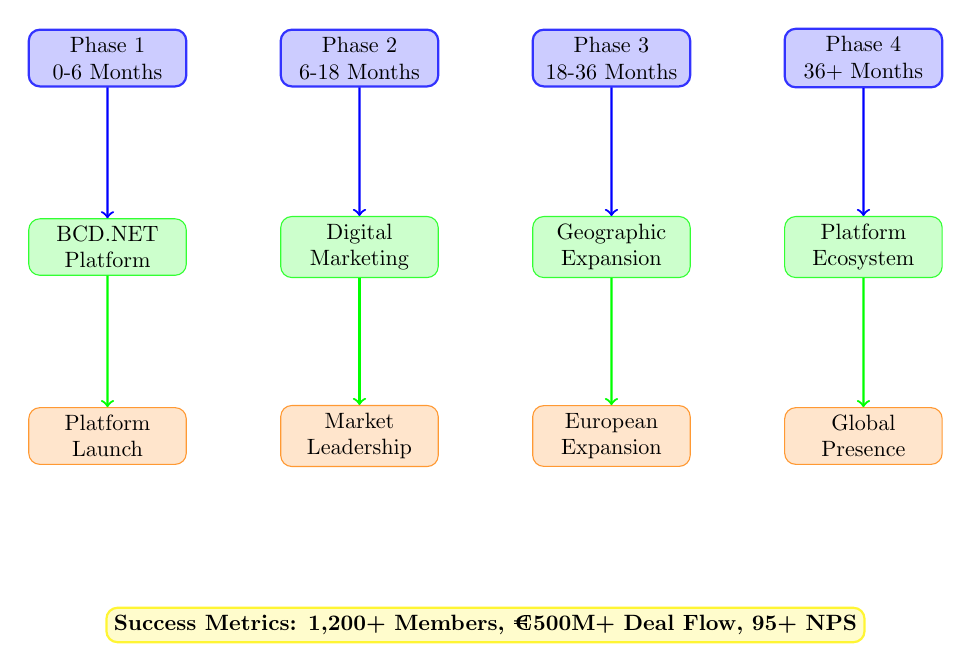
\begin{tikzpicture}[
    scale=0.8,
    transform shape,
    box/.style={rectangle, draw, rounded corners, minimum width=2.5cm, minimum height=0.8cm, align=center},
    phase/.style={box, fill=blue!20, draw=blue!80, thick},
    action/.style={box, fill=green!20, draw=green!80},
    timeline/.style={box, fill=orange!20, draw=orange!80},
    arrow/.style={->, thick}
]

% Timeline phases
\node[phase] (phase1) at (-6,3) {Phase 1\\0-6 Months};
\node[phase] (phase2) at (-2,3) {Phase 2\\6-18 Months};
\node[phase] (phase3) at (2,3) {Phase 3\\18-36 Months};
\node[phase] (phase4) at (6,3) {Phase 4\\36+ Months};

% Key actions
\node[action] (platform) at (-6,0) {BCD.NET\\Platform};
\node[action] (marketing) at (-2,0) {Digital\\Marketing};
\node[action] (expansion) at (2,0) {Geographic\\Expansion};
\node[action] (ecosystem) at (6,0) {Platform\\Ecosystem};

% Timeline milestones
\node[timeline] (milestone1) at (-6,-3) {Platform\\Launch};
\node[timeline] (milestone2) at (-2,-3) {Market\\Leadership};
\node[timeline] (milestone3) at (2,-3) {European\\Expansion};
\node[timeline] (milestone4) at (6,-3) {Global\\Presence};

% Connections
\draw[arrow, blue] (phase1) -- (platform);
\draw[arrow, blue] (phase2) -- (marketing);
\draw[arrow, blue] (phase3) -- (expansion);
\draw[arrow, blue] (phase4) -- (ecosystem);

\draw[arrow, green] (platform) -- (milestone1);
\draw[arrow, green] (marketing) -- (milestone2);
\draw[arrow, green] (expansion) -- (milestone3);
\draw[arrow, green] (ecosystem) -- (milestone4);

% Success metrics
\node[fill=yellow!20, draw=yellow!80, thick, rounded corners] at (0,-6) 
    {\textbf{Success Metrics: 1,200+ Members, €500M+ Deal Flow, 95+ NPS}};

\end{tikzpicture}
\caption{Implementation Roadmap and Success Metrics}
\label{fig:implementation-roadmap}
\end{figure}

\section{Strategic Recommendations}

Based on comprehensive market analysis and competitive research, the following strategic initiatives are recommended:

\subsection{Immediate Actions (0-6 months)}
\begin{enumerate}
    \item \textbf{Launch BCD.NET Platform}: Develop and launch the digital platform to enhance member engagement and provide additional value
    \item \textbf{Implement Digital Marketing Strategy}: Establish comprehensive digital marketing presence across LinkedIn, Instagram, and Twitter
    \item \textbf{Develop Thought Leadership Content}: Create regular content showcasing industry insights, member success stories, and deal flow opportunities
    \item \textbf{Strengthen Member Referral Program}: Enhance the referral system with better incentives and quality control measures
    \item \textbf{Optimize Website SEO}: Improve search engine optimization for better organic visibility in target markets
\end{enumerate}

\subsection{Strategic Initiatives (6-24 months)}
\begin{enumerate}
    \item \textbf{Geographic Expansion}: Explore opportunities to expand beyond DACH region into other European markets
    \item \textbf{Strategic Partnerships}: Develop partnerships with financial institutions, professional service firms, and technology providers
    \item \textbf{Technology Investment}: Invest in platform capabilities and digital tools to enhance member experience
    \item \textbf{Service Portfolio Expansion}: Develop additional retreat formats, educational programs, and investment opportunities
    \item \textbf{Investment Fund Development}: Consider establishing an investment fund or syndicate to enhance deal flow capabilities
\end{enumerate}

\subsection{Long-term Vision (2-5 years)}
\begin{enumerate}
    \item \textbf{Market Leadership}: Establish BCD as the leading premium networking platform in the DACH region
    \item \textbf{International Expansion}: Expand into key European markets with localized offerings
    \item \textbf{Platform Ecosystem}: Develop a comprehensive ecosystem of services and partnerships
    \item \textbf{Investment Platform}: Launch a full-featured investment platform for deal flow and co-investment opportunities
    \item \textbf{Educational Programs}: Develop certification and educational programs for members
\end{enumerate}

\section{Expected Outcomes}

The implementation of these strategic recommendations is expected to deliver:

\begin{itemize}
    \item \textbf{Member Growth}: Increase from 550+ to 1,200+ verified members
    \item \textbf{Deal Flow Expansion}: Grow from €100M+ to €500M+ annual transaction volume
    \item \textbf{Market Position}: Establish BCD as the premier DACH networking platform
    \item \textbf{Revenue Growth}: Achieve sustainable revenue growth through premium services
    \item \textbf{Competitive Advantage}: Maintain unique positioning in the market
\end{itemize}

The analysis demonstrates that bettercalldominik.com is well-positioned for significant growth in the premium business networking market, with a clear path to market leadership in the DACH region. 